\section{实验结果}

\subsection{工作曲线的绘制}

记录加入乙醇体积 $V_{\mathrm{EtOH}}$ 、加入环己烷体积 $V_{\mathrm{C y}}$, 称量小滴瓶空瓶质量 $m_0$ 、加入乙醇后质量 $m_1$ 、加入环己烷后质量 $m_2$, 计算乙醇的质量分数
$$
\chi_{\mathrm{EtOH}}=\frac{m_1-m_0}{m_2-m_0}=\frac{\Delta m_1}{\Delta m_2}
$$
经过计算得到各个溶液所对应的乙醇的质量分数,如表 \ref{tab:1} 所示。

\begin{table}[htbp]
    \centering
    \bicaption{各溶液中乙醇质量分数的计算}{Calculation of Ethanol Mass Fraction in Various Solutions}
    \begin{tabular}{ccccccccc}
        \toprule
        组分或编号 & $V_{\mathrm{EtOH}} / \mathrm{mL}$ & $V_{\mathrm{CyH}} / \mathrm{mL}$ & $m_0 / \mathrm{g}$ & $m_1 / \mathrm{g}$ & $m_2 / \mathrm{g}$ & $\Delta m_1 / \mathrm{g}$ & $\Delta m_2 / \mathrm{g}$ & $\chi_{\mathrm{EtOH}}$ \\
        \midrule 
        纯 \ce{CyH} & & & & & & & 0.0000 & 1.4218 \\
        1 & 1.00 & 8.00 & 28.4791 & 29.2517 & 35.4262 & 0.7726 & 6.9471 & 0.1112 \\
        2 & 2.00 & 7.00 & 25.1881 & 26.7333 & 30.5627 & 1.5452 & 5.3746 & 0.2875 \\
        3 & 3.00 & 6.00 & 29.5393 & 31.9158 & 36.5325 & 2.3765 & 6.9932 & 0.3398 \\
        4 & 4.00 & 5.00 & 35.5018 & 38.6453 & 42.5002 & 3.1435 & 6.9984 & 0.4492 \\
        5 & 5.00 & 4.00 & 28.2238 & 32.1272 & 35.2286 & 3.9034 & 7.0048 & 0.5572 \\
        6 & 6.00 & 3.00 & 29.5579 & 34.2048 & 36.5320 & 4.6469 & 6.9741 & 0.6663 \\
        7 & 7.00 & 2.00 & 32.9601 & 38.3195 & 39.8695 & 5.3594 & 6.9094 & 0.7757 \\
        8 & 8.00 & 1.00 & 32.3608 & 38.6483 & 39.4000 & 6.2875 & 7.0392 & 0.8932 \\
        纯 \ce{EtOH} & & & & & & & 1.0000  \\
        \bottomrule
        \end{tabular}
    \label{tab:1}
\end{table}

在恒温 $t=30.1\si{\celsius}$ 下分别测定不同乙醇质量分数的乙醇-环己烷溶液样品及纯乙醇、纯环已烷的折光率 $n$, 结果如表 \ref{tab:2} 所示。

\begin{table}[htbp]
    \centering
    \bicaption{各溶液中乙醇质量分数的计算}{Calculation of Ethanol Mass Fraction in Various Solutions}
    \begin{tabular}{cccccc}
        \toprule
            组分或编号 & $\chi_{\mathrm{EtOH}}$ & $n_1$ & $n_2$ & $n_3$ & $\bar{n}$\\
        \midrule 
            纯 \ce{CyH} & 0.0000 & 1.4200 & 1.4201 & 1.4202 & 1.4201 \\
            1 & 0.1112 & 1.4125 & 1.4127 & 1.4130 & 1.4127 \\
            2 & 0.2875 & 1.3992 & 1.3993 & 1.3995 & 1.3993 \\
            3 & 0.3398 & 1.3965 & 1.3967 & 1.3969 & 1.3967 \\
            4 & 0.4492 & 1.3879 & 1.3878 & 1.3879 & 1.3879 \\
            5 & 0.5572 & 1.3811 & 1.3807 & 1.3812 & 1.3810 \\
            6 & 0.6663 & 1.3734 & 1.3737 & 1.3739 & 1.3737 \\
            7 & 0.7757 & 1.3679 & 1.3677 & 1.3680 & 1.3679 \\
            8 & 0.8932 & 1.3604 & 1.3605 & 1.3605 & 1.3605 \\
            纯 \ce{EtOH} & 1.0000 & 1.3565 & 1.3566 & 1.3565 & 1.3565 \\
        \bottomrule
        \end{tabular}
    \label{tab:2}
\end{table}


使用python numpy.polyfit 的二次多项式拟合工作曲线,得到拟合公式:
\begin{equation}\label{eq:1}
    n = (0.01371\pm0.0026) \chi^2 - (0.07888\pm0.0027) \chi + (1.4208\pm0.0006);\quad R^2=0.99909
\end{equation}

画出折射率-乙醇质量分数的工作曲线,如图 \ref{fig:1} 所示。

\begin{figure}[htbp]
    \centering
    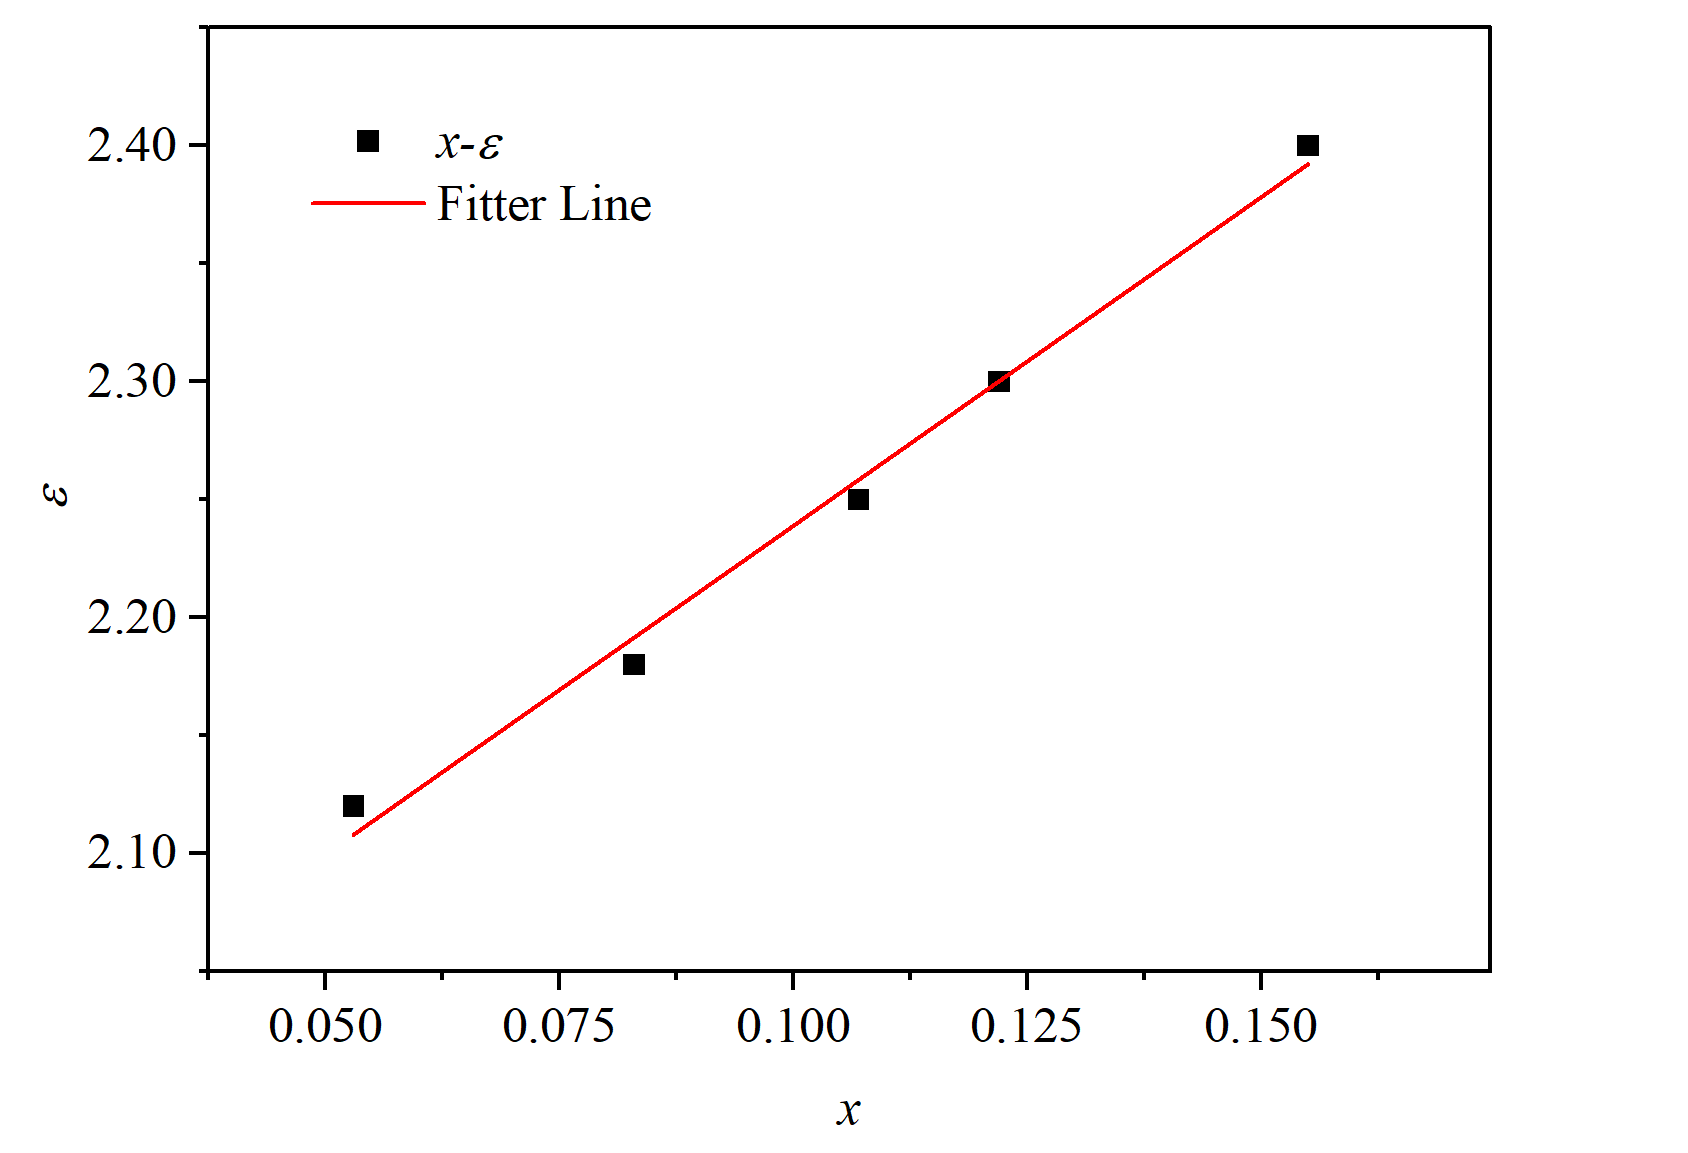
\includegraphics[width=.7\textwidth]{figures/1-1.png}
    \bicaption{乙醇-环己烷体系 $n-\chi_{\mathrm{EtOH}}$ 标准工作曲线}{Standard Working Curve of $n-\chi_{\mathrm{EtOH}}$ for Ethanol-Cyclohexane System}
    \label{fig:1}
\end{figure}

\subsection{沸点和两相成分的测定}


测定双液体系的沸点、支管冷凝液与恒沸液的折射率如表 \ref{tab:3},由于在取气相和液相时,沸腾的温度并不严格相同,因此我选取两个不同时间的沸点。

根据工作曲线 \eqref{eq:1} 这样的一个二次多项式,对于测出来的折射率,可以解析的给出这个方程根,也就是不同折射率下对应的乙醇质量分数 $\chi_{\mathrm{EtOH}}$。

\begin{table}[htbp]
    \centering
    \bicaption{乙醇-环己烷体系气液平衡时液相、气相组成计算数据}{Calculation Data of Liquid and Vapor Phase Compositions in EtOH-CyH System}
    \begin{tabular}{cccccccc}
    \toprule
     \ce{CyH} & \ce{EtOH} & $T_g$/\si{\celsius} & $n_g$ & $\chi_{\mathrm{EtOH,g}}$ &  $T_l$/\si{\celsius} & $n_l$ & $\chi_{\mathrm{EtOH,l}}$ \\
    \midrule
       0.0 &  20.0 & 78.43 & 1.3565 & 0.9835 & 78.42 & 1.3565 & 0.9835 \\
       1.0 &  20.0 & 76.10 & 1.3769 & 0.6245 & 75.89 & 1.3579 & 0.9567 \\
       2.0 &  20.0 & 74.62 & 1.3809 & 0.5606 & 74.99 & 1.3604 & 0.9098 \\
       4.0 &  20.0 & 71.26 & 1.3854 & 0.4908 & 71.29 & 1.3630 & 0.8621 \\
       7.0 &  20.0 & 68.40 & 1.3890 & 0.4364 & 68.41 & 1.3689 & 0.7580 \\
      10.0 &  20.0 & 67.66 & 1.3900 & 0.4215 & 67.11 & 1.3771 & 0.6212 \\
      14.0 &  20.0 & 66.24 & 1.3950 & 0.3483 & 66.22 & 1.3806 & 0.5653 \\
      19.0 &  20.0 & 65.63 & 1.3965 & 0.3268 & 65.80 & 1.3826 & 0.5340 \\
      \midrule
      20.0 &   0.0 & 81.00 & 1.4197 & 0.01412 & 81.10 & 1.4199 & 0.01157 \\
      20.0 &   0.2 & 78.88 & 1.4005 & 0.2702 & 78.91 & 1.4181 & 0.03458 \\
      20.0 &   0.4 & 76.12 & 1.3992 & 0.2884 & 76.19 & 1.4173 & 0.04486 \\
      20.0 &   0.9 & 69.97 & 1.3979 & 0.3068 & 70.25 & 1.4160 & 0.06165 \\
      20.0 &   1.4 & 68.02 & 1.3977 & 0.3097 & 68.12 & 1.4149 & 0.07594 \\
      20.0 &   3.4 & 65.64 & 1.3970 & 0.3196 & 65.65 & 1.4083 & 0.1632 \\
      20.0 &   8.4 & 65.58 & 1.3971 & 0.3182 & 65.38 & 1.3963 & 0.3296 \\
      20.0 &  13.4 & 65.36 & 1.3973 & 0.3154 & 65.62 & 1.3875 & 0.4589 \\
    \bottomrule
    \end{tabular}
    \label{tab:3}
\end{table}

根据表 \ref{tab:3} 中的数据,使用贝塞尔曲线(B-spline)进行插值绘制乙醇-环己烷体系的二组分相图,得到图 \ref{fig:2}。

\begin{figure}[htbp]
    \centering
    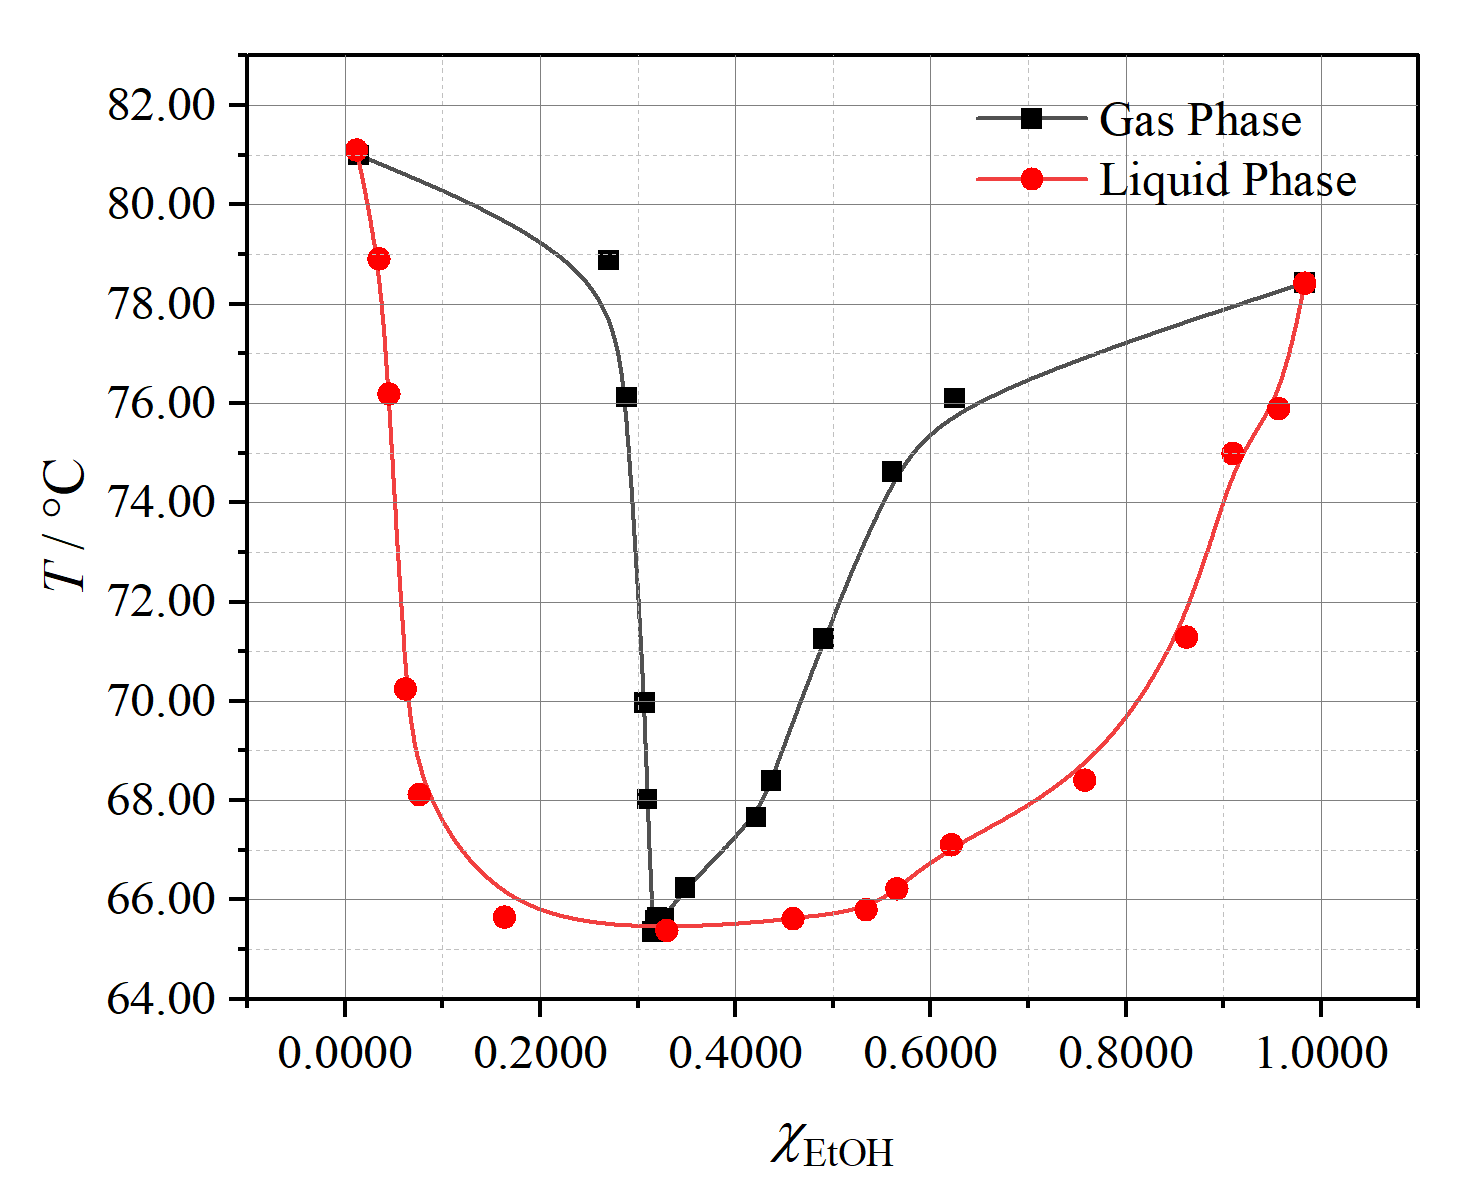
\includegraphics[width=.7\textwidth]{figures/1-2.png}
    \bicaption{乙醇-环己烷体系的二组分相图}{Binary Phase Diagram of the Ethanol-Cyclohexane System}
    \label{fig:2}
\end{figure}

根据图 \ref{fig:2},发现乙醇-环己烷体系存在一个最低恒沸点,将图 \ref{fig:2} 中的对应部分放大,得到图 \ref{fig:3},读取最低恒沸点的数据。

\begin{figure}[htbp]
    \centering
    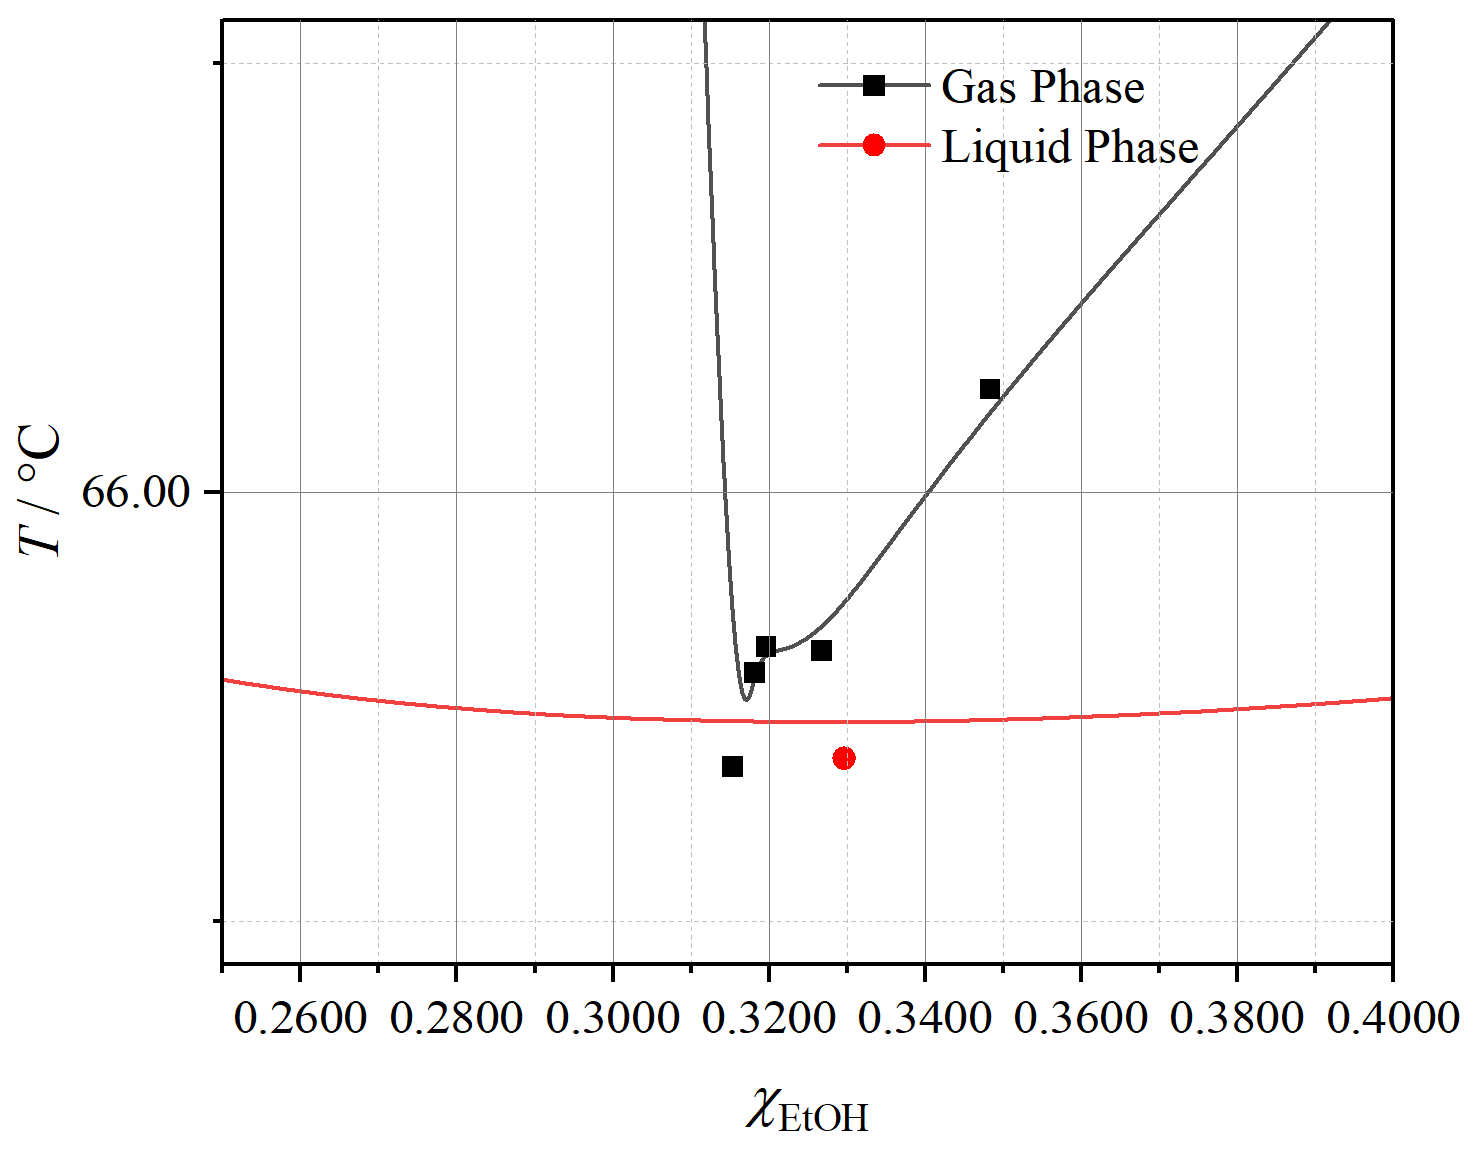
\includegraphics[width=.7\textwidth]{figures/1-3.png}
    \bicaption{乙醇-环己烷体系的二组分相图的最低恒沸点}{Minimum Azeotropic Point in the Binary Phase Diagram of the Ethanol-Cyclohexane System}
    \label{fig:3}
\end{figure}

根据图 \ref{fig:3},发现气相线与液相线并不重合,这可能是由于测定误差和贝塞尔拟合曲线的误差导致的,因此,我们首先选取气相线的最低点 $\chi_{\rm{EtOH}}=0.3171, T_g = 65.52\si{\celsius}$),然后根据其 $\chi_{\rm{EtOH}}$ 值找到液相线对应的沸点 $T_l = 65.47\si{\celsius}$,取 $T_g,T_l$ 的平均作为最低恒沸点的温度 $T$:
\[
T = \frac{T_g+T_l}{2}=65.49\si{\celsius}
\]




